\documentclass[a4paper,leqno]{article}
\usepackage[utf8]{inputenc}
\usepackage{lmodern}
\usepackage{microtype}
\usepackage[inline]{enumitem}

\usepackage{siunitx}
\usepackage{multirow}
\usepackage{subcaption}

\usepackage[english]{babel}
\usepackage[autostyle, english=british]{csquotes}
\MakeOuterQuote{"}

\usepackage{commath}
\usepackage{amsmath}
\usepackage{amsthm}
\usepackage{amssymb}
\usepackage{mathtools}

\usepackage{pgfplots}
\pgfplotsset{compat=1.11}
\usepgfplotslibrary{fillbetween}
\usetikzlibrary{patterns}

\newcommand*{\SectorRadius}{1.5ex}
\newcommand*{\SectorHalfAngle}{45}
\newcommand*{\SectorLineWidth}{.4pt}

\newcommand*{\sector}{%
  \begin{pgfpicture}
    \pgfpathmoveto{\pgforigin}%
    \pgfpathlineto{\pgfpointpolar{90-(\SectorHalfAngle)}{\SectorRadius}}%
    \pgfarc{90-(\SectorHalfAngle)}{90+\SectorHalfAngle}{\SectorRadius}%
    \pgfpathclose
    \pgfsetlinewidth{\SectorLineWidth}%
    \pgfusepath{stroke}%
  \end{pgfpicture}%
}

\usepackage{hyperref}

\usepackage[margin=1in]{geometry}
\usepackage{changepage}
\usepackage{titlesec}
\titleformat{\section}{\normalfont\Large\bfseries\centering}{Section~\thesection:}{1em}{}

\def\signed #1{{\leavevmode\unskip\nobreak\hfil\penalty50\hskip2em
  \hbox{}\nobreak\hfil(#1)%
  \parfillskip=0pt \finalhyphendemerits=0 \endgraf}}
\newsavebox\mybox
\newenvironment{aquote}[1]
  {\savebox\mybox{#1}\begin{quote}}
  {\signed{\usebox\mybox}\end{quote}}

% Augmented matrices.
\makeatletter
\renewcommand*\env@matrix[1][*\c@MaxMatrixCols c]{%
  \hskip -\arraycolsep
  \let\@ifnextchar\new@ifnextchar
  \array{#1}}
\makeatother

%--------grstep
% For denoting a Gauss' reduction step.
% Use as: \grstep{\rho_1+\rho_3} or \grstep[2\rho_5 \\ 3\rho_6]{\rho_1+\rho_3}
\newcommand{\grstep}[2][\relax]{%
   \ensuremath{\mathrel{
       {\mathop{\longrightarrow}\limits^{#2\mathstrut}_{
                                     \begin{subarray}{l} #1 \end{subarray}}}}}}
\newcommand{\swap}{\leftrightarrow}


\swapnumbers
\numberwithin{equation}{section}
\newtheorem{thm}[equation]{Theorem}
\newtheorem{lem}[equation]{Lemma}
\newtheorem{cor}[equation]{Corollary}
\newtheorem{prp}[equation]{Proposition}
\theoremstyle{definition}
\newtheorem{defn}[equation]{Definition}
\newtheorem{notation}[equation]{Notation}
\newtheorem{ex}[equation]{Example}
\newtheorem{exercise}[equation]{Exercise}
\newtheorem{alg}[equation]{Algorithm}
\theoremstyle{remark}
\newtheorem{rem}[equation]{Remark}

\newcommand{\df}[1]{\textbf{#1}}
\newcommand{\T}{\mathrm{T}}
\newcommand{\F}{\mathrm{F}}
\newcommand{\IndSet}{\mathbf{I}}
\DeclareMathOperator{\cis}{cis}
\DeclareMathOperator{\versin}{versin}
\DeclareMathOperator{\cvs}{cvs}
\DeclareMathOperator{\exsec}{exsec}
\DeclareMathOperator{\excsc}{excsc}
\DeclareMathOperator{\crd}{crd}

\title{Level Three Trigonometry}
\author{Alex Elzenaar}
\date{\today}

\begin{document}
\maketitle
\tableofcontents
\section*{Preface}
These notes present a brief overview of the trigonometry required for Level 3 Calculus. We
mainly treat the subject from a functional viewpoint.

\titleformat{\section}{\clearpage\titlerule[0.8pt]\vspace{0.5ex}\normalfont\Large\bfseries\centering}{Section~\thesection:}{1em}{}[{\titlerule[0.8pt]}]
\let\oldsection\section
\renewcommand\section{\clearpage\oldsection}
\section{Definitions}
\begin{notation}
  We will denote points by uppercase letters; the line through the points $ X $ and $ Y $ is denoted $ XY $, and the length of the
  segment between $ X $ and $ Y $ will be denoted $ \abs{XY} $. If $ O $, $ A $, and $ B $ are points, then $ \angle AOB $ denotes
  the angle that starts at the ray $ OA $ and is measured anticlockwise to the ray $ OB $. The area of a figure $ \mathfrak{F} $ is
  denoted by $ \mathcal{A}(\mathfrak{F}) $.
\end{notation}

\begin{center}
  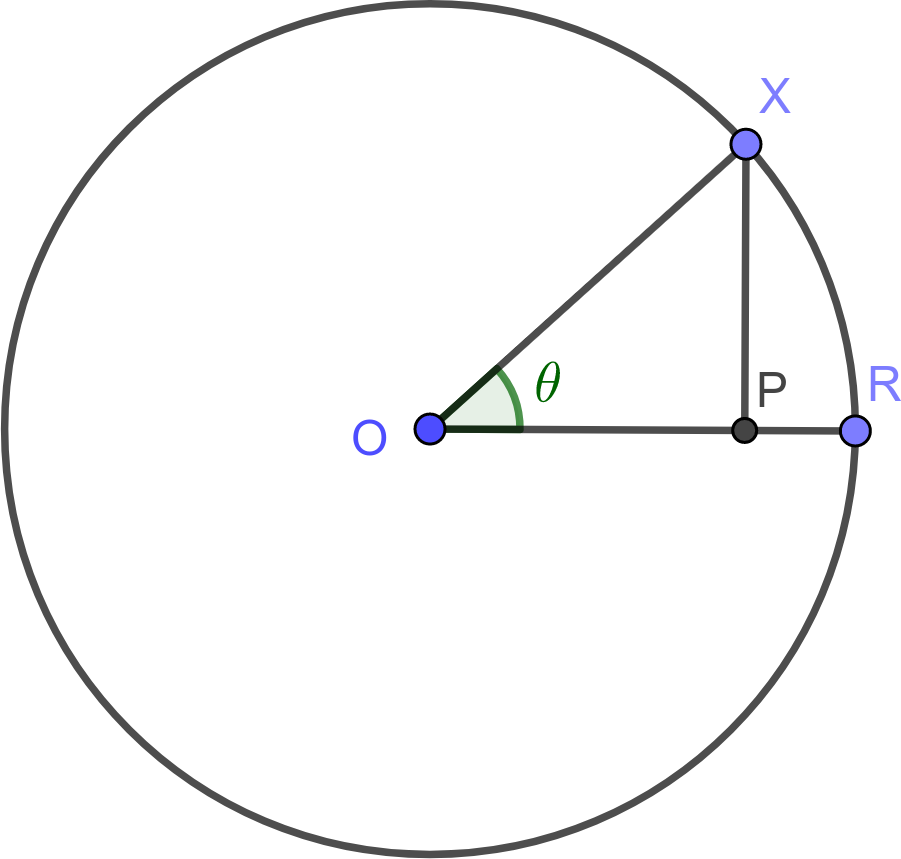
\includegraphics[width=0.3\textwidth]{fndefinitions}
\end{center}

\begin{defn}\label{defn:trig1}
  Consider a unit circle with centre $ O $ and radius $ OR $. Let $ X $ be any point on the circle, such that the angle between $ OR $ and $ OX $
  is $ \theta $ (i.e. such that the proportion of the circumference between $ R $ and $ X $ is $ \theta/2\pi $). Draw the line through $ X $,
  perpendicular to the radius $ OR $ and cutting the latter at $ P $. Then we define two functions of $ \theta $ as follows, called the \df{sine} and \df{cosine}
  functions respectively, for all $ 0 \leq \theta < \pi/2 $:-
  \begin{gather}
    \sin(\theta) = \abs{PX}\\
    \cos(\theta) = \abs{OP}.
  \end{gather}
\end{defn}

It is customary to drop the parentheses around the argument of trigonometric functions if it is a single term; for
example, $ \sin \theta $ simply means $ \sin(\theta) $. We adopt this convention whenever it is unambiguous.

It is also customary to write $ \sin^2 \theta $ in place of $ (\sin \theta)^2 $, and in general $ \sin^n \theta $
for $ (\sin \theta)^n $ whenever $ n $ is a positive integer.

Clearly, we also have $ \sin 0 = 0 $ and $ \cos 0 = 1 $.

We then extend the domains of definition of sine and cosine to the entire range $ 0 \leq \theta < 2\pi $, as follows:
\begin{equation}\label{tab:extend1}
\begin{tabular}{c|c|c|c}
  & $ \frac{\pi}{2} \leq \theta < \pi $ & $ \pi \leq \theta < \frac{3\pi}{2} $ & $ \frac{3\pi}{2} \leq \theta < 2\pi $\\\hline
  $ \sin \theta = $ & $ \sin(\pi - \theta) $ & $ -\sin(\theta - \pi)$ & $-\sin(2\pi - \theta) $\\
  $ \cos \theta = $ & $ -\cos(\pi - \theta) $ & $ - \cos (\theta - \pi) $ & $ \cos(2\pi - \theta) $.
\end{tabular}
\end{equation}

Drawing the graphs of $ y = \sin x $ (red) and $ y = \cos x $ (blue) for $ 0 \leq x < 2\pi $, we obtain the
following picture.
\begin{center}
  \fbox{\begin{tikzpicture}
    \begin{axis}[
      axis lines = center,
      ymax = 1.5, ymin = -1.5,
      xtick={1.5708, 3.14159, 4.7124, 6.28},
      xticklabels={$\frac{\pi}{2}$,$\pi$,$\frac{3\pi}{2}$,$2\pi$},
      xlabel = $ x $,
      ylabel = $ y $
    ]
      \addplot[domain = 0:2*pi, color = red] {sin(deg(x))};
      \addplot[domain = 0:2*pi, color = blue] {cos(deg(x))};
    \end{axis}
  \end{tikzpicture}}
\end{center}

Finally, we extend the domains of definition to the entire real line by declaring that for all real $ \theta $, the identities
\begin{gather}
  \sin \theta = \sin (\theta + 2n\pi)\text{ and}
  \cos \theta = \cos (\theta + 2n\pi)
\end{gather}
hold (where $ n $ is any integer). This simply implies that the graphs of the two functions repeat every $ 2\pi $; hence the graphs
as drawn above can be extended as far as we like in either direction by just making shifted copies of the bit we already drew.
\begin{center}
  \fbox{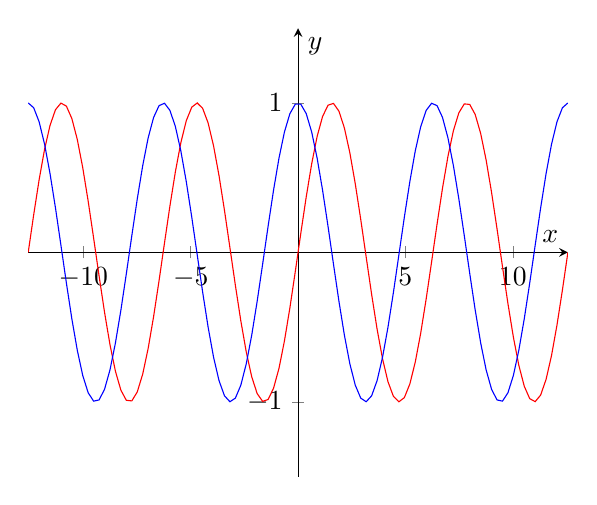
\begin{tikzpicture}
    \begin{axis}[
      axis lines = center,
      ymax = 1.5, ymin = -1.5,
      xtick={},
      xlabel = $ x $,
      ylabel = $ y $
    ]
      \addplot[domain = -4*pi:4*pi, color = red, samples=100] {sin(deg(x))};
      \addplot[domain = -4*pi:4*pi, color = blue, samples=100] {cos(deg(x))};
    \end{axis}
  \end{tikzpicture}}
\end{center}

\begin{exercise}
  Consider the unit circle again, call $ PX $ positive whenever $ X $ lies above the $ OR $ axis and negative whenever $ X $ lies below that
  axis. Then call $ OP $ positive whenever $ P $ lies on the segment $ OR $ and negative when $ P $ lies on the opposite side of $ R $. Show
  that if we define $ \sin \theta $ and $ \cos \theta $ by $ PX $ and $ OP $ respectively for all $ 0 \leq \theta < 2\pi $, keeping signs
  consistent, then the resulting functions agree with our definition above.
\end{exercise}

\begin{prp}\label{thm:basicids}
  The following identities always hold.
  \begin{enumerate}
    \item $ -1 \leq \sin \theta \leq 1 $ and $ -1 \leq \cos \theta \leq 1 $ for all $ \theta $.
    \item $ \sin 2n\pi = 0 $ and $ \cos 2n\pi = 1 $ for all integers $ n $.
    \item $ \sin^2 \theta + \cos^2 \theta = 1 $ for all $ \theta $.
    \item $ \sin (-\theta) = -\sin \theta $ and $ \cos (-\theta) = \cos \theta $ for all $ \theta $.
    \item $ \cos \theta = \sin (\theta + \pi/2) $.
  \end{enumerate}
\end{prp}
\begin{proof}\leavevmode
  \begin{enumerate}
    \item For $ 0 \leq \theta < \pi/2 $, the two functions are defined using the lengths $ PX $ and $ OP $ which
          are positive and always less than 1. For all other values of $ \theta $, the functions are defined in
          terms of the values on this interval and are not scaled beyond a negative sign; so both functions are
          bounded above by 1 and below by $ -1 $.
    \item $ \sin 2n\pi = \sin(0 + 2n\pi) = \sin 0 = 0 $. A similar calculation holds for cosine.
    \item When $ 0 \leq \theta < \pi/2 $, the statement follows from an application of Pythagoras' theorem
          to the right triangle $ OPX $. When $ \pi/2 \leq \theta < \pi $,
            \begin{displaymath}
              \sin^2 \theta + \cos^2 \theta = \sin^2(\pi - \theta) + (-\cos (\pi - \theta))^2 = 1
            \end{displaymath}
            (since $ 0 \leq \pi - \theta < \pi/2 $); similar arguments show that the statement holds for all $ 0 \leq \theta < 2\pi $.
            If $ \theta $ is not in this range, then $ \theta = \theta' + 2n\pi $ for some integer $ n $ and some $ \theta' $ that
            does lie in that range; since $ \sin (\theta' + 2n\pi) = \sin \theta' $, and $ \cos (\theta' + 2n\pi) = \cos \theta' $, we
            can apply what we have already proved in this case as well.
    \item Note that $ \sin(-\theta) = \sin(2\pi - \theta) = -\sin \theta $, and $ \cos(-\theta) = \cos(2\pi - \theta) = \cos \theta $ (by
          the final column of table \ref{tab:extend1}).
    \item Suppose $ 0 \leq \theta < \pi/2 $. Then, considering the following diagram, we perform some angle-pushing.
          \begin{center}
            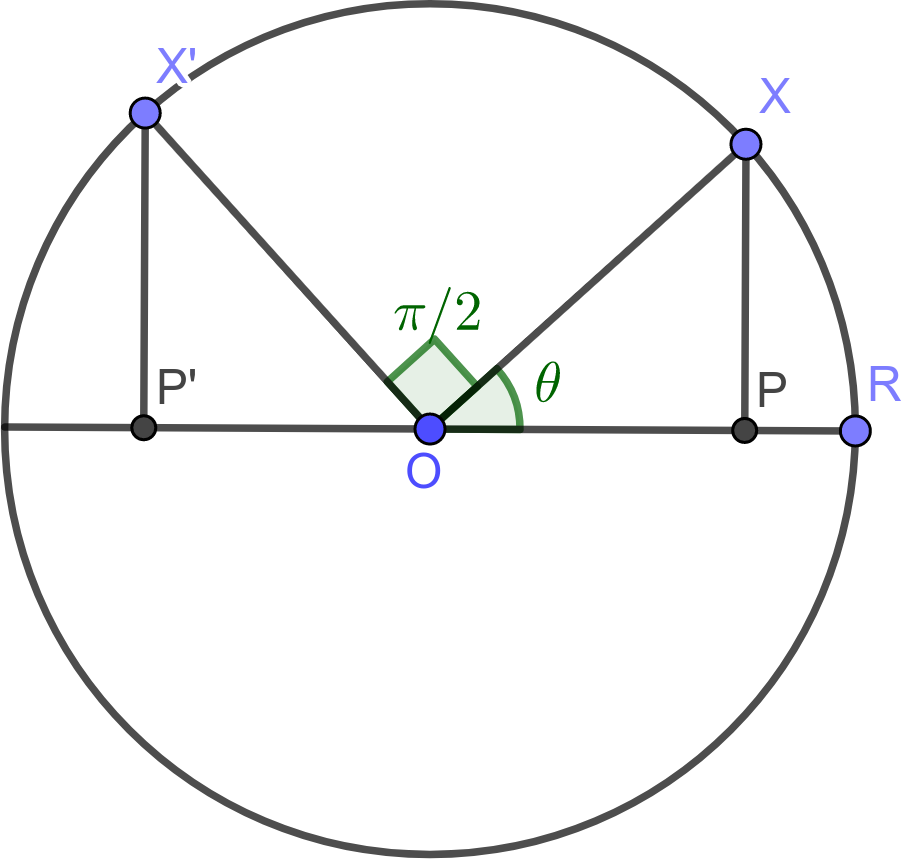
\includegraphics[width=0.3\textwidth]{shifting}
          \end{center}
          The angle $ \angle X'OP' $ has magnitude $ \frac{\pi}{2} - \theta $; hence the other angle in the right
          triangle $ X'OP' $ has magnitude $ \theta $ (since the angle-sum of triangles is $ \pi $). The two triangles
          $ XOP $ and $ X'OP' $ share all three of their angles and so are similar, and share an edge length (the radius
          of the circle) and so are equal, with lengths $ \abs{X'P'} = \abs{OP} $ and $ \abs{OP'} = \abs{XP} $. But $ \abs{X'P'} = \sin(\theta + \pi/2) $,
          and $ \abs{OP} = \cos \theta $; hence the proposition holds in this case.

          If $ \pi/2 \leq \theta < \pi $, then $ \pi \leq \theta + \pi/2 < 3\pi/2 $ and $ \sin(\theta + \pi/2) = -\sin(\theta + \pi/2 - \pi) $;
          then (applying the case we have already proved) $ -\sin(\theta - \pi/2) = -\cos(\theta - \pi) = \cos \theta $ as required. We extend
          the proof to all $ 0 \leq \theta < 2\pi $ using similar arguments, and then conclude it holds for all $ \theta $ by periodicity.
  \end{enumerate}
\end{proof}

\begin{thm}
  If $ ABC $ is a right triangle such that the right angle is at $ C $, and $ \alpha $ is the interior angle at $ A $, then
    \begin{gather}
      \sin \alpha = \frac{\abs{BC}}{\abs{AB}} = \frac{\text{opposite}}{\text{hypotenuse}} \text{ and}\\
      \cos \alpha = \frac{\abs{AC}}{\abs{AB}} = \frac{\text{adjacent}}{\text{hypotenuse}}.
    \end{gather}
\end{thm}
\begin{proof}
  Construct a similar triangle $ A'B'C' $ by scaling every length of $ ABC $ by $ 1/\abs{AB} $; drawing a circle
  with radius 1 and centre $ A $, we see that $ \abs{B'C'} = \cos \alpha $ and $ \abs{A'C'} = \sin \alpha $ (taking
  the base radius to be $ A'C' $ and applying our original definition \ref{defn:trig1}). But $ \abs{B'C'} = \abs{BC}/\abs{AB} $,
  and $ \abs{A'C'} = \abs{AC}/\abs{AB} $, so we are done.
\end{proof}

Instead of pushing the definitions further, we take all the properties we know that sine and cosine have and move on to
defining some more trigonometric functions. Consider the following diagram.

\begin{center}
  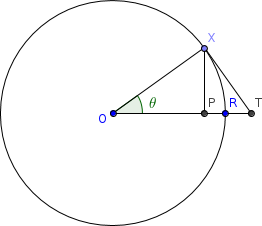
\includegraphics[width=0.3\textwidth]{tangent}
\end{center}

\begin{thm}
  If $ OXP $ is drawn in a unit circle as in the diagram, and the tangent line to the circle at $ X $ is drawn to meet the line $ OR $ at
  some point $ T $, then $ \abs{XT} = \frac{\sin \theta}{\cos \theta} $.
\end{thm}
\begin{proof}
  I claim that $ XOT $ is similar to $ POX $. This is proved by noticing that both triangles
  contain a right angle and share the angle of measure $ \theta $. Hence $ \frac{\abs{XT}}{\abs{XO}} = \frac{\abs{XP}}{\abs{OP}} $;
  but $ \abs{XO} = 1 $, $ \abs{XP} = \sin \theta $, and $ \abs{OP} = \cos \theta $, so we are done.
\end{proof}

Motivated by this theorem, we make the following
\begin{defn}
  The \df{tangent} function is the function $ \tan $ that is defined by
  \begin{displaymath}
    \tan \theta = \frac{\sin \theta}{\cos \theta}
  \end{displaymath}
  for all $ \theta \neq \frac{\pi}{2}n $ where $ n $ is an odd integer (since $ \cos \frac{\pi}{2}n $ is zero for odd $ n $).
\end{defn}

The following theorem is useful in calculus.
\begin{thm}
  For $ -\pi/2 < \theta < \pi/2 $, $ 1 < \frac{\sin x}{x} < \cos x $. In particular, as $ x \to 0 $, $ \frac{\sin x}{x} \to 1 $.
\end{thm}
\begin{center}
  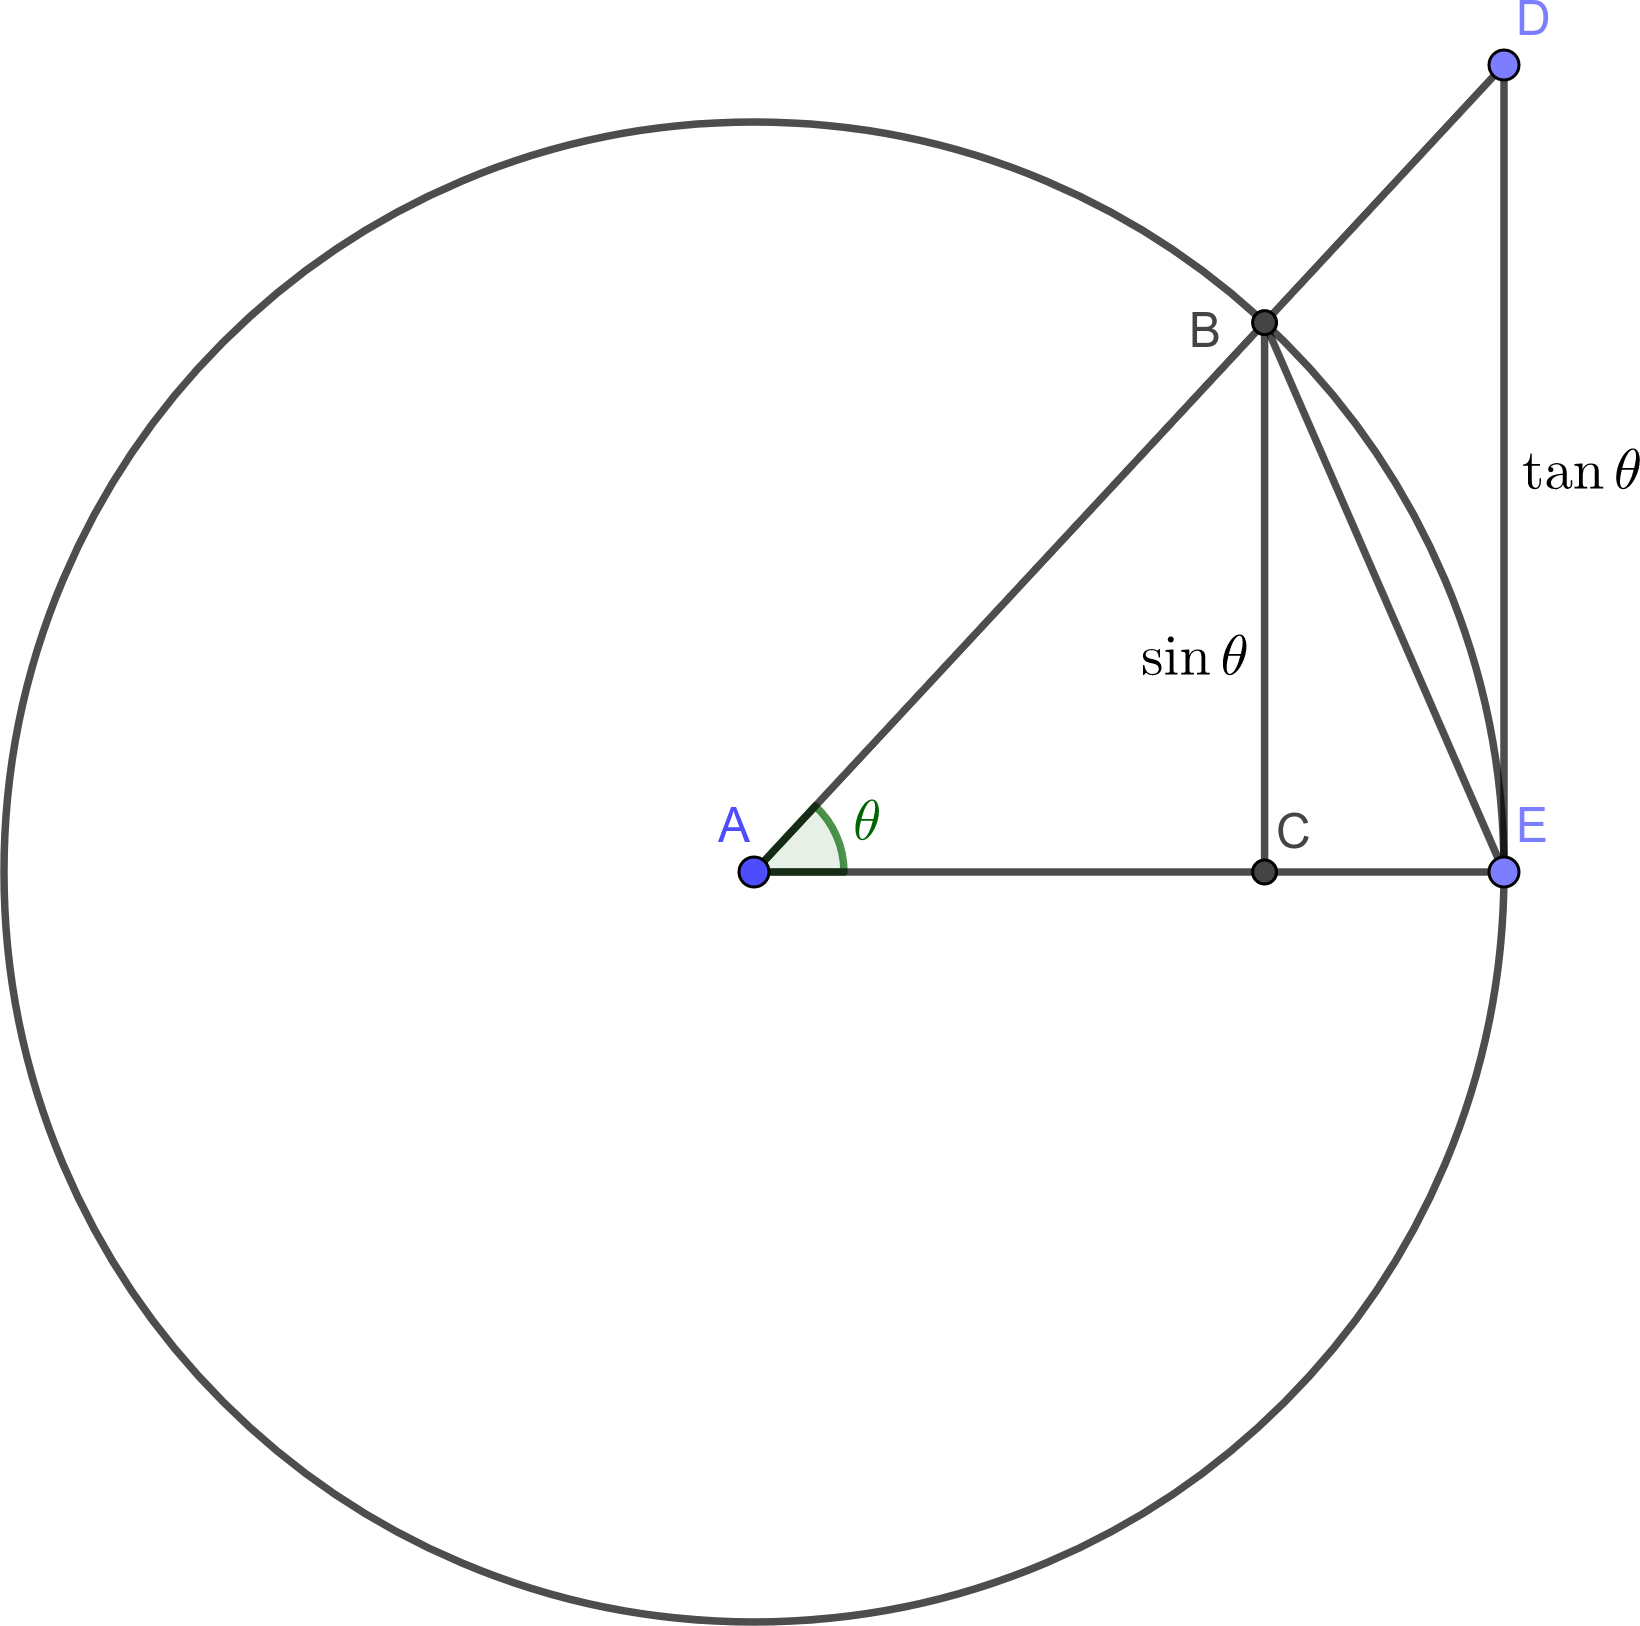
\includegraphics[width=0.3\textwidth]{sinelimit}
\end{center}
\begin{proof}
  For $ \theta > 0 $, we can use the diagram above. We have that $\mathcal{A}(\triangle ABC) = \frac{1}{2} \sin \theta $,
  that $ \mathcal{A}(\sector ABC) = \frac{\theta}{2} $, and that $ \mathcal{A}(ADE) = \frac{1}{2}\tan \theta $. By comparison
  of these areas, we have $ \frac{1}{2}\sin \theta \leq \frac{1}{2}\theta \leq \frac{1}{2}\tan \theta $ and
  hence $ 1 \leq \frac{\theta}{\sin \theta} \leq \cos \theta $.

  If $ \theta < 0 $ then $ -\theta > 0 $; we then have $ \frac{\theta}{\sin \theta} = \frac{-\theta}{\sin(-\theta)} $. Applying
  the part we have already proved, we have $ 1 \leq \frac{-\theta}{\sin(-\theta)} \leq \frac{1}{\cos(-\theta)} $. Replacing $ \cos(-\theta) $
  with $ \cos \theta $, allowed because of proposition \ref{thm:basicids}, we have the desired result for negative $ \theta $.
\end{proof}

\section{Taxonomy of Functions}
For the remainder of these notes, we only consider angles $ 0 \leq \theta < 2\pi $ unless otherwise stated. This is because
all of the interesting theory occurs in this case, and extending results to arbitrary $ \theta $ is tedious and doesn't present
any inherent complexity. The reader is invited to keep in mind our definitions from above, and to fill in on her own those
places where a negative sign or some other modification may be needed to make a result hold in general.

Consider now the following diagram based on our definitions above, where the tangent line $ XT $ to the unit circle has been
extended to meet the vertical line at $ B $; we also drop a perpendicular line from $ X $ onto the vertical line at $ A $.
Our goal is to work out how most of the new lengths we can play with depend on the trigonometric functions we have already
defined; the reader is encouraged to annotate the diagram with the names of the various functions, like $ \tan $, as they
are defined. A complete diagram is given at the end of the section.
\begin{center}
  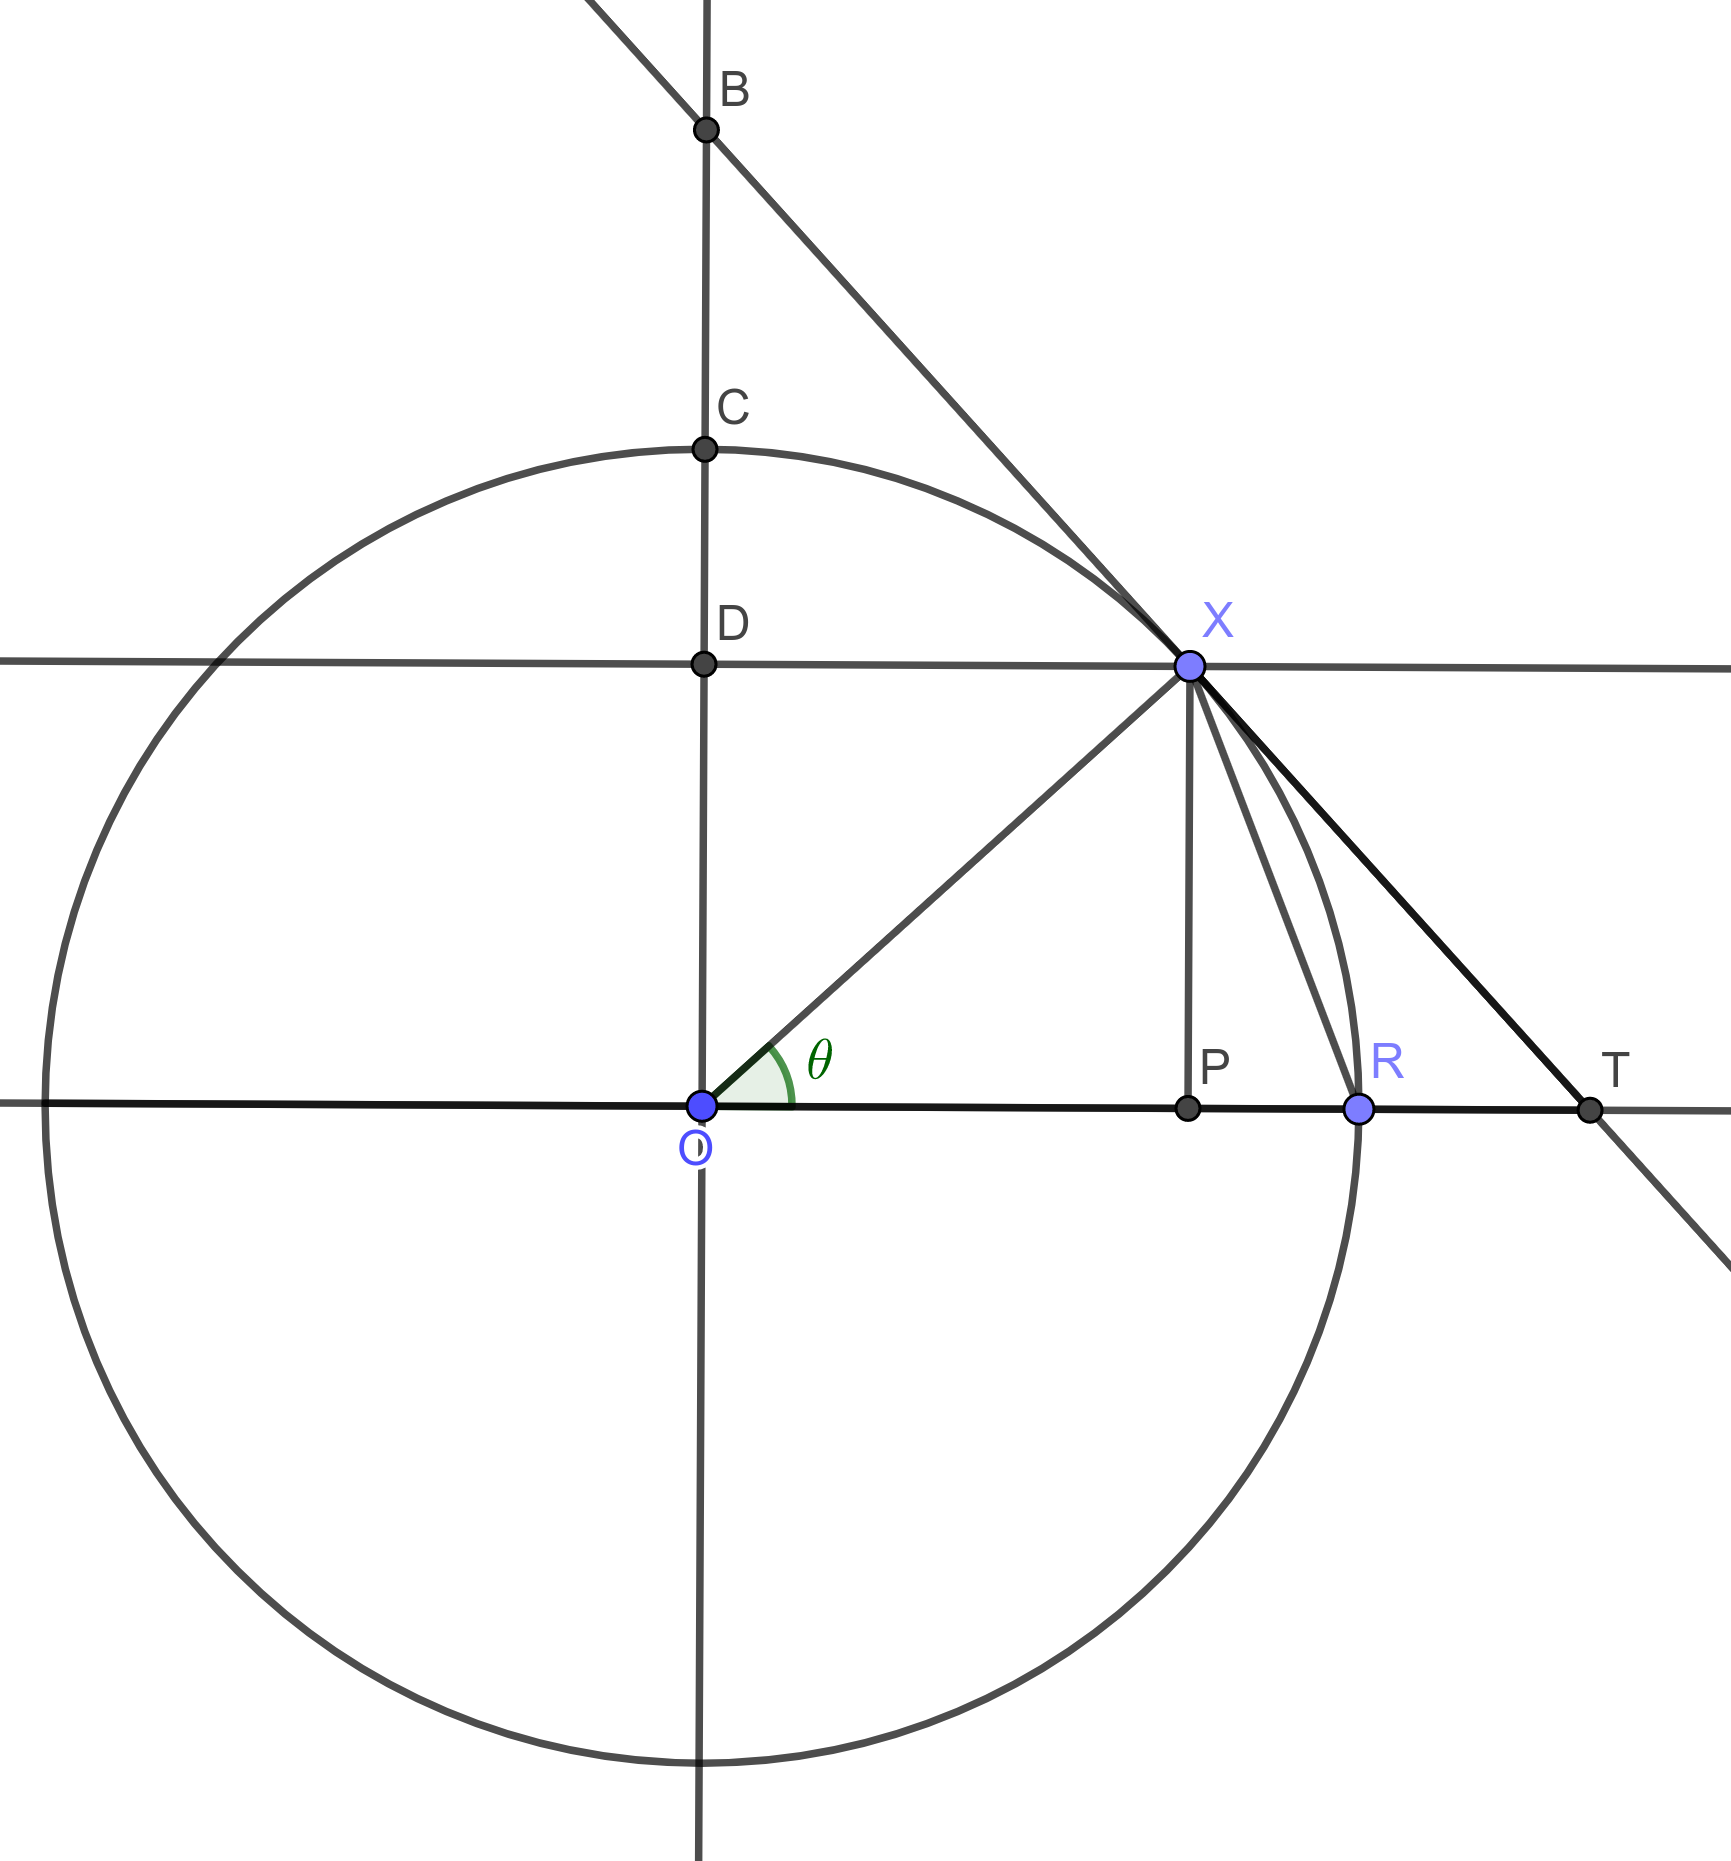
\includegraphics[width=0.7\textwidth]{taxonomy}
\end{center}

\subsection{Reciprocal Functions}
Firstly, we calculate the length of $ OT $. Consider the triangle $ OXT $; we can calculate its area in two different ways,
recalling that the area of a triangle is one half of the base times the height.
\begin{displaymath}
  \mathcal{A}(OXT) = \frac{1}{2}\abs{XT}\abs{OX} = \frac{1}{2}\abs{OT}\abs{PX}
\end{displaymath}
However, $ \abs{XT} = \tan \theta $, $ \abs{OX} = 1 $, and $ \abs{PX} = \sin \theta $. Hence we
have $ \tan \theta = \abs{OT}\sin \theta $; but $ \tan \theta = \frac{\sin \theta}{\cos \theta} $,
so $ \abs{OT} = \frac{1}{\cos \theta} $.
\begin{defn}
  The \df{secant} function is defined by $ \sec \theta = \abs{OT} = \frac{1}{\cos \theta} $.
\end{defn}

We next calculate $ \abs{BX} $. Note that $ DBX $ and $ PXT $ are similar triangles, and so $ \frac{\abs{BX}}{\abs{DX}} = \frac{\abs{XT}}{\abs{PT}} $.
Substituting in what we know, this becomes
\begin{equation}\label{eqn:cotan1}
  \frac{\abs{BX}}{\cos \theta} = \frac{\tan \theta}{\abs{PT}};
\end{equation}
but $ PXT $ is a right triangle and so, applying the Pythagorean theorem,
\begin{displaymath}
  \abs{PT} = \sqrt{\tan^2 \theta - \sin^2 \theta} = \sqrt{\frac{\sin^2 \theta}{\cos^2 \theta} - \sin^2 \theta} = \sin \theta \sqrt{\frac{1}{\cos^2 \theta} - 1},
\end{displaymath}
or (substituting into equation \ref{eqn:cotan1})
\begin{displaymath}
  \frac{\abs{BX}}{\cos \theta} = \frac{\tan\theta}{\sin\theta \sqrt{\frac{1}{\cos^2 \theta} - 1}}.
\end{displaymath}
Cancelling $ \tan \theta = \sin \theta/\cos \theta $,
\begin{displaymath}
  \abs{BX} = \frac{1}{\sqrt{\frac{1}{\cos^2 \theta} - 1}}.
\end{displaymath}
To simplify further, recall that $ \sin^2 \theta + \cos^2 \theta = 1 $, and so (dividing by $ \cos^2 \theta $)
\begin{equation}\label{eqn:tansecid}
  \tan^2 \theta + 1 = \frac{1}{\cos^2 \theta} = \sec^2 \theta.
\end{equation}
Hence $ \abs{BX} = \frac{1}{\sqrt{\tan^2 \theta}} = \frac{1}{\tan \theta} $.

\begin{defn}
  The \df{cotangent} function is defined by $ \cot \theta = \abs{BX} = \frac{1}{\tan \theta} $.
\end{defn}

Our next trick is to calculate $ \abs{OB} $. Again, we use similar triangles: $ OBT $ is similar to $ PXT $. In
particular, $ \frac{\abs{OB}}{\abs{OT}} = \frac{\abs{PX}}{\abs{PT}} $. But $ \abs{OT} = \sec \theta $, $ \abs{PX} = \sin \theta $,
and $ \abs{PT} = \sin \theta \sqrt{\sec^2 \theta - 1} = \sin \theta \tan \theta = \frac{\sin^2 \theta}{\cos \theta} $. Hence
\begin{displaymath}
  \abs{OB} = \abs{OT} \frac{\abs{PX}}{\abs{PT}} = \sec \theta \frac{\sin \theta}{\sin^2 \theta/\cos \theta} = \frac{1}{\sin \theta}.
\end{displaymath}

\begin{defn}
  The \df{cosecant} function is defined by $ \csc \theta = \abs{OB} = \frac{1}{\sin \theta} $.
\end{defn}

\begin{exercise}
  Show the pretty identity that $ \sec^2 \theta \csc^2 \theta = \sec^2 \theta \csc^2 \theta $. (Hint: apply Pythagoras to $ OBT $.)
\end{exercise}

\subsection{Historical Functions}
\begin{exercise}\leavevmode
  \begin{enumerate}
    \item By applying Pythagoras' theorem to $ BOT $, show that $ \cot^2 \theta + \tan^2 \theta + 2 = \csc^2 \theta + \sec^2 \theta $,
          and conclude by equation \ref{eqn:tansecid} that $ \cot^2 \theta + 1 = \csc^2 \theta $.
    \item By imitating the proof of equation \ref{eqn:tansecid} (i.e. using the identity $ \sin^2 \theta + \cos^2 \theta = 1 $), show
          that $ \cot^2 \theta + 1 = \csc^2 \theta $.
  \end{enumerate}
\end{exercise}

A few easy lengths follow, which only have names for historical reasons.
\begin{defn}\leavevmode
  \begin{enumerate}
    \item The \df{versine} function is defined by $ \versin \theta = \abs{PR} = 1 - \cos \theta $.
    \item The \df{coversine} function is defined by $ \cvs \theta = \abs{CD} = 1 - \sin \theta $.
    \item The \df{exsecant} function is defined by $ \exsec \theta = \abs{RT} = \sec \theta - 1 $.
    \item The \df{excosecant} function is defined by $ \excsc \theta = \abs{BC} = \csc \theta - 1$.
  \end{enumerate}
\end{defn}

\begin{exercise}
  Taking inspiration from our proofs above showing that the reciprocal trig functions correspond
  to lengths, show the following identities involving the historical trig functions.
  \begin{enumerate}
    \item $ \exsec \theta = \excsc \theta \tan \theta $
    \item $ (\versin \theta)(\cvs \theta) = \sin^2 \theta $
  \end{enumerate}
\end{exercise}

\subsection{Chords}
Finally, we compute $ \abs{XR} $. We have
\begin{displaymath}
  \abs{XR}^2 = \sin^2 \theta + \versin^2 \theta = \sin^2 \theta + (1 - \cos \theta)^2 = \sin^2 \theta + 1 - 2\cos \theta + \cos^2 \theta = 2 - 2\cos \theta.
\end{displaymath}

\begin{defn}
  The \df{chord} function is defined by $ \crd \theta = \abs{XR} = \sqrt{2 - 2\cos \theta} $.
\end{defn}

We can calculate this function in a different way using the cosine rule which we learned last year.

\begin{center}
  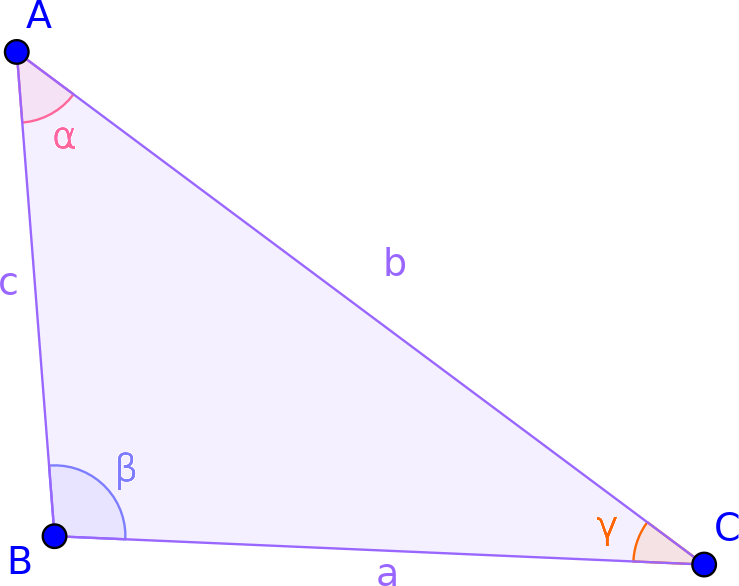
\includegraphics[width=0.2\textwidth]{trisines}
\end{center}

\begin{thm}[Law of cosines]
  If $ ABC $ is a triangle, labeled as in the picture, then $ c^2 = a^2 + b^2 - 2ab \cos \gamma $.
\end{thm}

Rather than repeat the standard proof, I will give one based on the intersecting chord theorem.
\begin{thm}
  Suppose that $ A $, $ B $, $ C $, and $ D $ lie on a circle, and the lines $ AB $ and $ CD $ intersect at
  some point $ X $ inside the circle. Then $ \abs{AX} \abs{XB} = \abs{CX} \abs{XD} $.
\end{thm}
\begin{center}
  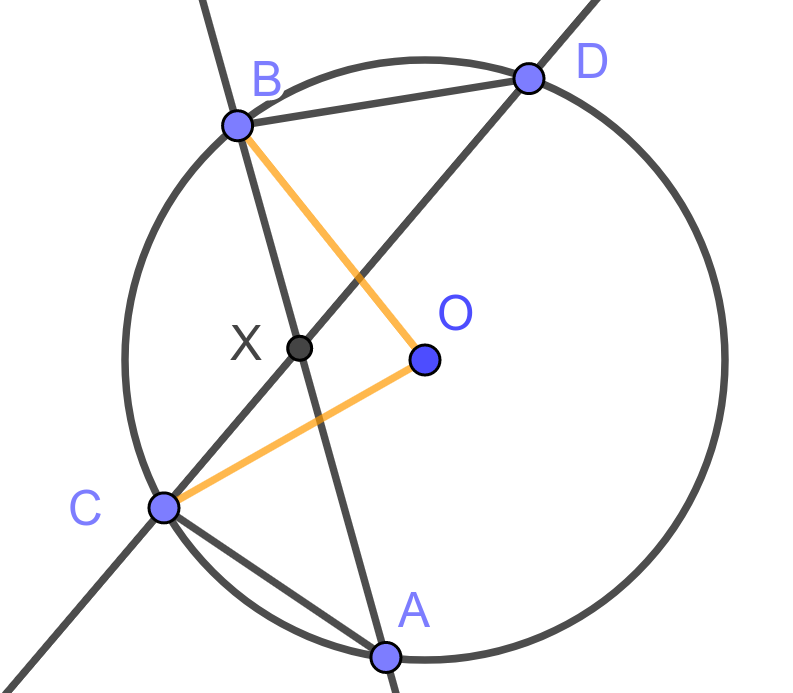
\includegraphics[width=0.3\textwidth]{ichords}
\end{center}
\begin{proof}
  I claim that $ BXD $ and $ CXA $ are similar. Clearly the two angles $ \angle DXB $ and $ \angle CXA $ are
  equal, because they are opposite. By the inscribed angle theorem, $ \angle BOC = 2\angle BDC = 2\angle BAC $
  because all three are subtended by the chord $ BC $. Hence both triangles have two equal angles, and are similar.
  The result follows from taking the side ratios $ \frac{AX}{CX} = \frac{XD}{XB} $.
\end{proof}

The following proof of the law of cosines is due to Kung.\footnote{``Proof without Words: The law of cosines via Ptolemy's Theorem.'' \textit{Mathematics Magazine}, 65(2), p. 103. doi:10.1080/0025570X.1992.11995990}
\begin{center}
  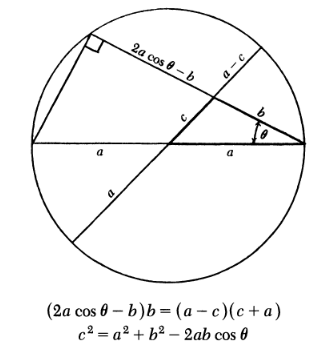
\includegraphics[width=0.4\textwidth]{cosinelawproof}
\end{center}

Then $ \crd \theta = \sqrt{1^2 + 1^2 - 2\cdot1\cdot1\cdot \cos \theta} = \sqrt{2 - 2\cos \theta} $ as before.

\subsection{Summary of the Taxonomy}
\begin{center}
  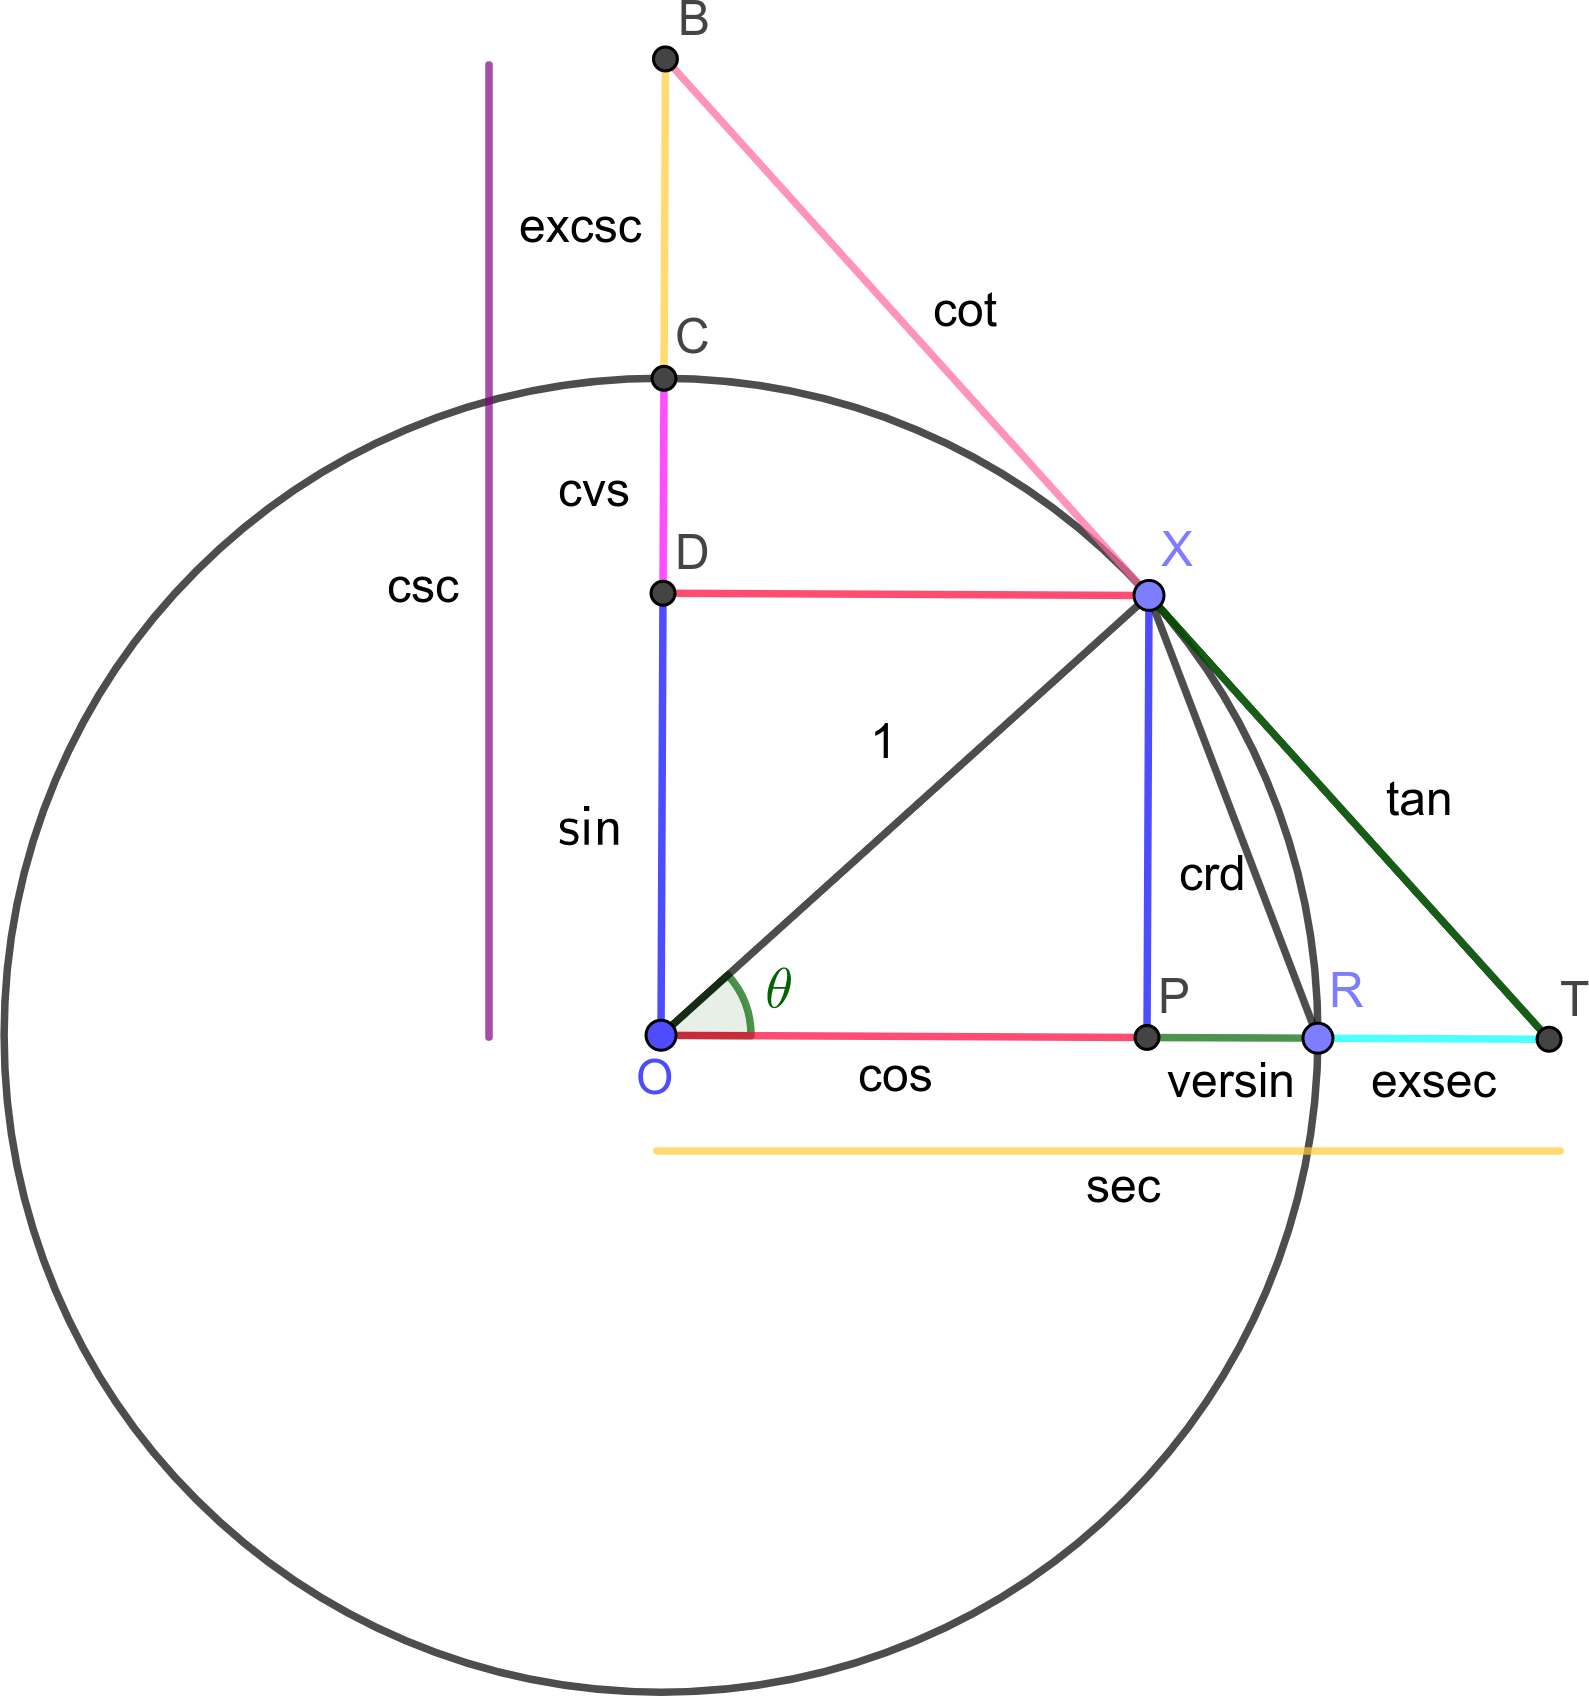
\includegraphics[width=0.5\textwidth]{taxonomyall}
\end{center}
We have the following definition, which summarises all the definitions we have made.
\begin{defn}\leavevmode
  \begin{enumerate}
    \item \textbf{Basic Functions}
      \begin{enumerate}
        \item $ \sin \theta = \abs{PX} $ (sine)
        \item $ \cos \theta = \abs{OP} $ (cosine)
        \item $ \tan \theta = \abs{XT} = \frac{\sin \theta}{\cos \theta} $ (tangent)
      \end{enumerate}
    \item \textbf{Reciprocal Functions}
      \begin{enumerate}
        \item $ \csc \theta = \abs{OB} = \frac{1}{\sin\theta} $ (cosecant)
        \item $ \sec \theta = \abs{OT} = \frac{1}{\cos\theta} $ (secant)
        \item $ \cot \theta = \abs{BX} = \frac{1}{\tan\theta} = \frac{\cos\theta}{\sin\theta} $ (cotangent)
      \end{enumerate}
    \item \textbf{Historical Functions}
      \begin{enumerate}
        \item $ \versin \theta = \abs{PR} = 1 - \cos \theta $ (versine)
        \item $ \cvs \theta = \abs{CD} = 1 - \sin \theta $ (coversine)
        \item $ \exsec \theta = \abs{RT} = \sec \theta - 1 $ (exsecant)
        \item $ \excsc \theta = \abs{BC} = \csc \theta - 1$ (excosecant)
      \end{enumerate}
    \item \textbf{Other Functions}
      \begin{enumerate}
        \item $ \crd \theta = \abs{RX} = \sqrt{2 - 2\cos \theta} $ (chord)
      \end{enumerate}
  \end{enumerate}
\end{defn}
Of these, the basic functions and the reciprocal functions are the most useful.

We also have the following identities.
\begin{thm}\leavevmode
  \begin{enumerate}
    \item $ \sin^2 \theta + \cos^2 \theta = 1 $
    \item $ \tan^2 \theta + 1 = \sec^2 \theta $
    \item $ 1 + \cot^2 \theta = \csc^2 \theta $
  \end{enumerate}
\end{thm}

\section{Identity Fishing}
Recall that if we consider the function $ \exp $ which maps $ x \to e^x $, then we have the addition rule $ \exp(x + y) = \exp(x) \exp(y) $. Our
goal in this section is to derive similar rules for the basic trigonometric functions.

\begin{thm}\leavevmode\label{thm:sumids}
  Suppose $ \alpha $ and $ \beta $ are angles. Then:
  \begin{enumerate}
    \item $ \sin(\alpha + \beta) = \sin \alpha \cos \beta + \cos \alpha \sin \beta $
    \item $ \cos(\alpha + \beta) = \cos \alpha \cos \beta - \sin \alpha \sin \beta $
  \end{enumerate}
\end{thm}
\begin{proof}
  We prove the formulae for angles in the range $ 0 \leq \alpha < \pi/2 $ and $ 0 \leq \beta \pi/2 $, and this
  result can be generalised to all $ \theta $ using the same methods we have used before.

  For cosine, consider the following diagram.\footnote{Both this proof and the one given in the exercise below are due to Leonard M. Smiley, University of Alaska Anchorage, \url{http://math.uaa.alaska.edu/~smiley/trigproofs.html} (retrieved via Archive.org on 14 Sept 2018).}
  \begin{center}
    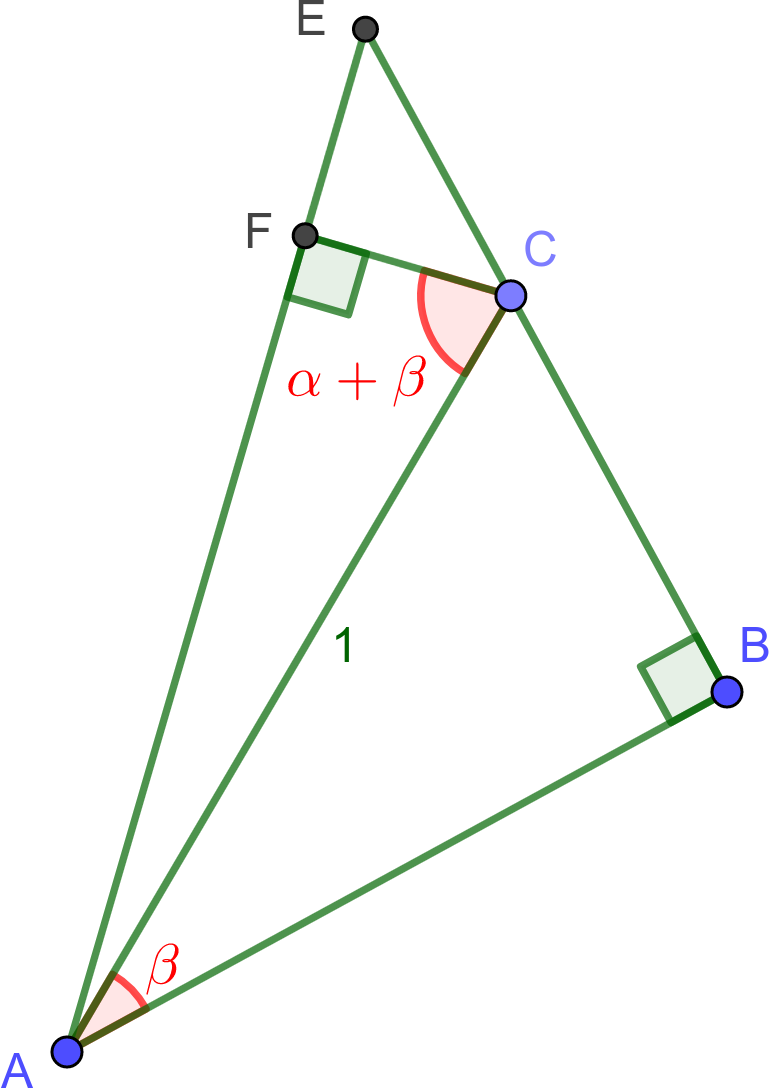
\includegraphics[width=0.3\textwidth]{cosinesum}
  \end{center}
  We have two triangles, where $ ABC $ has an angle $ \beta $ and hypotenuse $ \abs{AC} = 1 $. From $ C $ we measure an angle $ \alpha + \beta $,
  and extend this line to meet a line from $ C $ at a right angle (so both interior angles at $ F $ are right). Hence $ \abs{AB} = \cos\beta $,
  $ \abs{BC} = \sin \beta $, and $ \abs{FC} = \cos(\alpha + \beta) $. I claim that the interior angle at $ E $ is simply $ \alpha $; this
  can be seen by writing the interior angle of $ EFC $ at $ C $ as $ \pi - (\alpha + \beta) + (\pi/2 - \beta) = \pi/2 - \alpha $ and then
  using the fact that the angle sum of a triangle is $ \pi $. Using this fact and the length of $ FC $, we have that
  \begin{displaymath}
    \abs{EC} = \frac{\cos (\alpha + \beta)}{\sin \alpha}.
  \end{displaymath}
  Then by taking side ratios of the large triangle $ ABE $ we have $ \frac{\abs{AB}}{\abs{BE}} = \frac{\sin \alpha}{\cos \alpha} $, and hence
  \begin{displaymath}
    \frac{\sin \alpha}{\cos \alpha} = \frac{\cos \beta}{\frac{\cos (\alpha + \beta)}{\sin \alpha} + \sin \beta},
  \end{displaymath}
  which is rearranged to obtain $ \cos(\alpha + \beta) = \cos \alpha \cos \beta - \sin \alpha \sin \beta $ as required.
\end{proof}

\begin{exercise}
  Use the following diagram and an analagous argument to derive the sum formula for sine.
  \begin{center}
    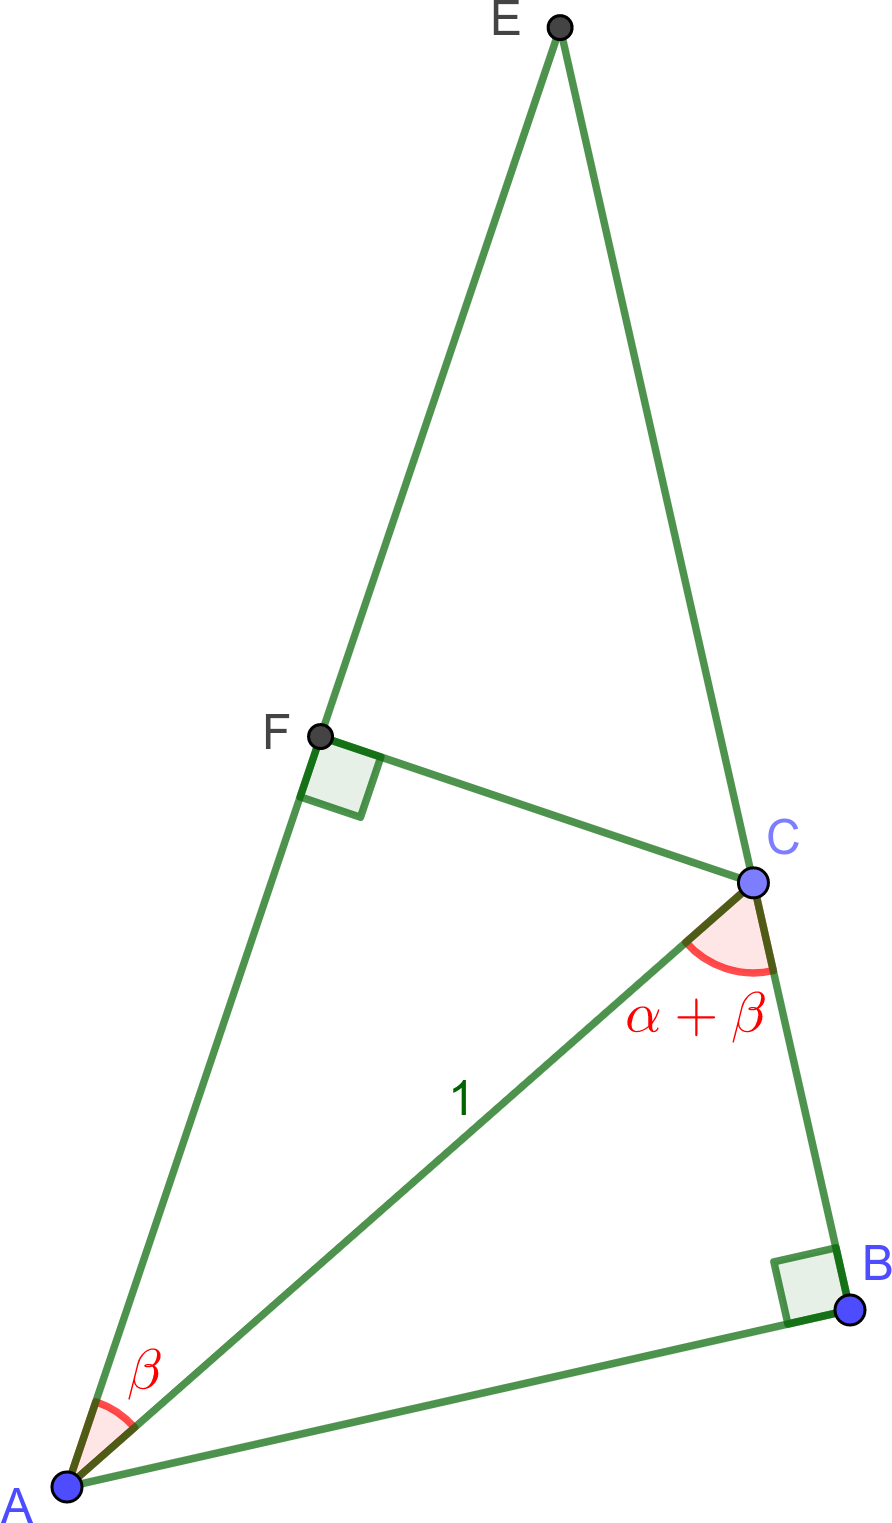
\includegraphics[width=0.3\textwidth]{sinesum}
  \end{center}
  Hint: write down $ \abs{AF} $, $ \abs{FC} $, and $ \abs{AB} $. Then show that the interior angle at $ E $ is still $ \alpha $,
  and that $ \abs{EF} = \frac{\sin\beta \cos\alpha}{\sin \alpha} $. Finally, $ \sin \alpha = \frac{\abs{AB}}{\abs{EF}} $.
\end{exercise}

\begin{cor}
  We also have the following identities:-
  \begin{enumerate}
    \item $ \sin(\alpha - \beta) = \sin \alpha \cos \beta - \cos \alpha \sin \beta $
    \item $ \cos(\alpha - \beta) = \cos \alpha \cos \beta + \sin \alpha \sin \beta $
    \item $ \tan(\alpha + \beta) = \frac{\tan \alpha + \tan \beta}{1 - \tan \alpha \tan \beta} $
    \item $ \tan(\alpha - \beta) = \frac{\tan \alpha - \tan \beta}{1 + \tan \alpha \tan \beta} $
    \item $ \sin(2\alpha) = 2 \sin \alpha \cos \alpha $
    \item $ \cos(2\alpha) = \cos^2 \alpha - \sin^2 \alpha = 1 - 2\sin^2 \alpha = 2\cos^2 \alpha - 1 $.
  \end{enumerate}
\end{cor}
\begin{proof}
  For (1) and (2), simply replace $ \beta $ with $ -\beta $ in theorem \ref{thm:sumids} and apply part (4) of proposition \ref{thm:basicids}.

  For (3), write $ \tan(\alpha + \beta) = \frac{\sin(\alpha + \beta)}{\cos(\alpha + \beta)} $, apply parts (1) and (2), and simplify. Then (4)
  follows in a similar way to (1) and (2) (noting that $ \tan (-\theta) = -\tan \theta $).

  For (5) and (6), set $ \beta = \alpha $ and apply theorem \ref{thm:sumids}.
\end{proof}

\begin{exercise}
  Show the following product identities hold.
  \begin{enumerate}
    \item $ 2 \sin \alpha \cos \beta = \sin(\alpha + \beta) + \sin(\alpha - \beta) $
    \item $ 2 \cos \alpha \sin \beta = \sin(\alpha + \beta) - \sin(\alpha - \beta) $
    \item $ 2 \cos \alpha \cos \beta = \cos(\alpha + \beta) + \cos(\alpha - \beta) $
    \item $ 2 \sin \alpha \sin \beta = \cos(\alpha - \beta) - \cos(\alpha + \beta) $ (note reversed $ \pm $)
  \end{enumerate}
  Find an expression for $ \tan \alpha \tan \beta $ in terms of $ \cos $.
\end{exercise}
\begin{exercise}
  Show the following half-angle identities hold.
  \begin{enumerate}
    \item $ \sin^2 \left(\frac{\alpha}{2}\right) = \frac{1 - \cos \alpha}{2} $
    \item $ \cos^2 \left(\frac{\alpha}{2}\right) = \frac{1 + \cos \alpha}{2} $
    \item $ \tan^2 \left(\frac{\alpha}{2}\right) = \frac{1 - \cos \alpha}{1 + \cos \alpha} $
  \end{enumerate}
  To remove the power of two on the left, we must take the square root of the right in each case. This root
  can have two signs: it may be positive, or negative, depending on the value of $ \alpha $. Classify all the
  relevant cases. (For which $ \alpha $ is $ \sin \alpha/2 $ positive, and for which $ \alpha $ is it negative? Repeat for all three.)
\end{exercise}
\begin{exercise}
  Show the following sum identities hold.
  \begin{enumerate}
    \item $ \sin \alpha + \sin \beta = 2\sin \frac{\alpha + \beta}{2} \cos \frac{\alpha - \beta}{2} $
    \item $ \sin \alpha - \sin \beta = 2\cos \frac{\alpha + \beta}{2} \sin \frac{\alpha - \beta}{2} $
    \item $ \cos \alpha + \cos \beta = 2\cos \frac{\alpha + \beta}{2} \cos \frac{\alpha - \beta}{2} $
    \item $ \cos \alpha - \cos \beta = -2\sin \frac{\alpha + \beta}{2} \sin \frac{\alpha - \beta}{2} $ (note negative)
  \end{enumerate}
\end{exercise}

Finally, we prove the following aesthetic identity.
\begin{thm}
  If $ x + y + z = \pi $, then $ \sin 2x + \sin 2y + \sin 2z = 4\sin x \sin y \sin z $.
\end{thm}
\begin{proof}
  First, note that since $ z = \pi - x - y $, we have $ \sin z = \sin(x + y) $ and $ \cos z = -\cos(x + y) $. This follows
  from the facts $ \sin \theta = \sin(\pi - \theta) $ and $ \cos \theta = -\cos(\pi - \theta) $ which can be easily seen
  from symmetry in the case $ 0 \leq \theta < \pi/2 $ using the unit circle (figure), and then for all other $ \theta $ by
  applying table \ref{tab:extend1} and proposition \ref{thm:basicids}.
  \begin{center}
    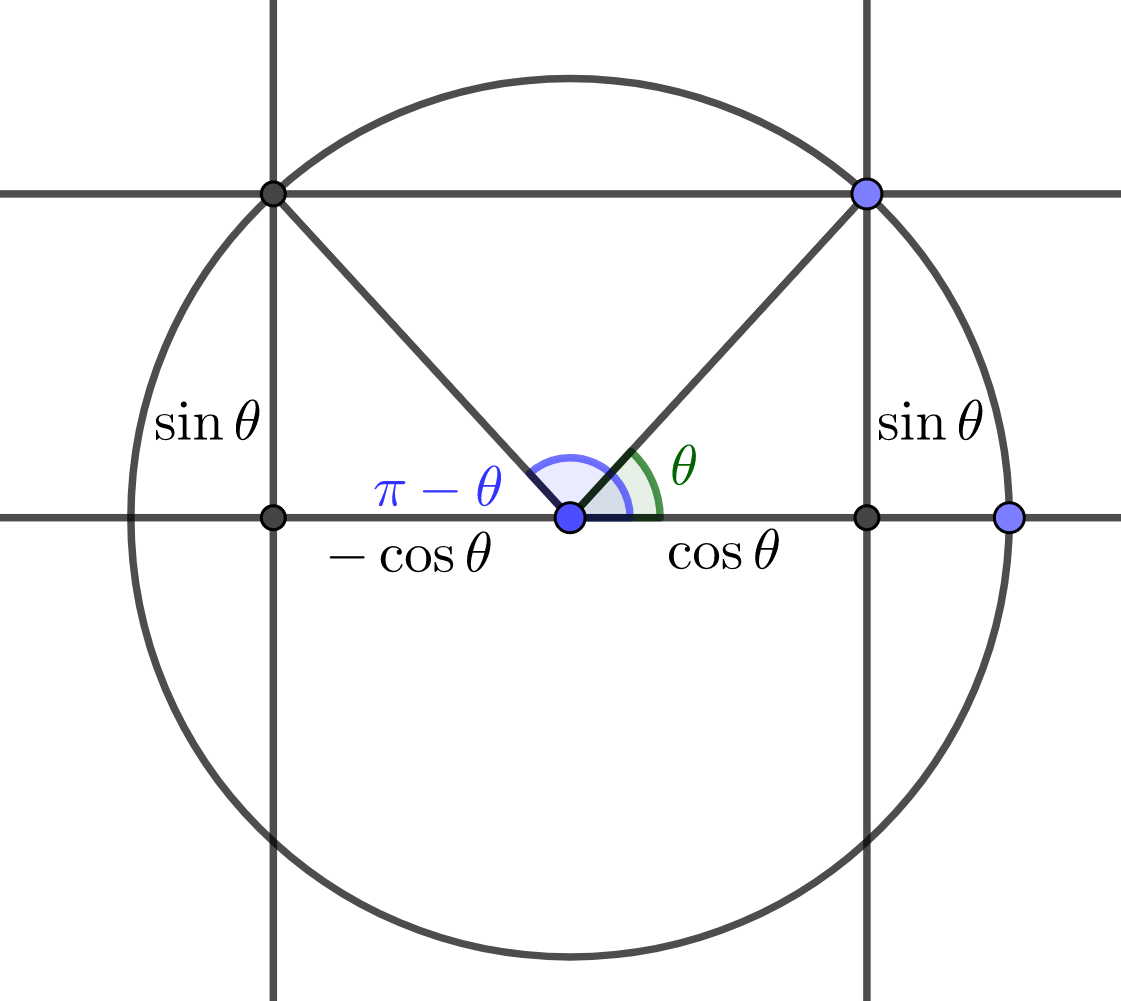
\includegraphics[width=0.3\textwidth]{piminus}
  \end{center}
  Then we argue as follows.
  \begin{align*}
    \sin 2x + \sin 2y + \sin 2x &= 2\sin(x + y)\cos(x - y) + 2\sin z \cos z\\
                                &= 2\sin z \cos(x - y) - 2\sin z \cos(x + y)\\
                                &= 2\sin z [\cos(x - y) - \cos(x + y)]\\
                                &= 2\sin z [\cos x \cos y + \sin x \sin y - \cos x \cos y + \sin x \sin y]\\
                                &= 4\sin x \sin y \sin z.
  \end{align*}
\end{proof}

\section{Inverse Functions}

\section{Periodic Models}

\end{document}
